\documentclass[a4paper,11pt]{style-esi/td}

\usepackage{style-esi/licence}
\usepackage{style-esi/exercice}
\usepackage{style-esi/exemple}
\usepackage{style-esi/question}
\usepackage{style-esi/tutoriel}
\usepackage{style-esi/listing}
\usepackage{style-esi/images}
\usepackage{style-dev1/dev1}

\begin{document}

\seance{0}{Lost material}
\entete
\titre
\ccbysa{esi-dev1-list@he2b.be}
\lastedit

\bigskip
\tableofcontents

%===================
\section{Rechercher (dans) des fichiers}
%====================

	Lorsqu'on commence à avoir beaucoup de fichiers,
	il arrive qu'on ne sache plus trop bien où se trouve un fichier
	ou quel fichier contient un texte particulier.
	Les commandes \samp{find} et \samp{grep} sont là pour nous aider.

	%===================
	\subsection{Rechercher un fichier}
	%====================

		La commande \samp{find} permet de chercher des fichiers
		dans le système de fichiers en fonction de critères : 
		son nom, sa taille, sa date de création\dots

		\begin{theorie}{find}
			\kbd{find dossierOùChercher critèreDeRecherche...}
			cherche dans le dossier indiqué (et tous les sous dossiers)
			les fichiers qui respectent tous les critères indiqués.
			Par défaut, la commande affiche le nom des fichiers trouvés.

			Parmi les critères citons :
			\begin{itemize}
				\item \kbd{-name nomfichier}
			\end{itemize}
        \end{theorie}
        
%=================================
\section{Les variables d'environnement}  
%=================================

	\subsection{Introduction}
	%========================

		\begin{theorie}{Variable d'environnement}
			Une \textbf{variable d'environnement} 
			est une variable associée à votre shell 
			contenant un texte qui est accessible 
			par toutes les applications que vous lancez. 
			Généralement, elle permet de configurer certaines applications, 
			d'en modifier le comportement.
		\end{theorie}	

		\begin{theorie}{Manipuler une variable d'environnement}
			Si \samp{VARENV} est une variable d'environnement :
			\begin{itemize}
			\item \kbd{export VARENV=valeur} crée une nouvelle variable à la valeur donnée.
			\item \kbd{VARENV=valeur} modifie la valeur d'une variable existante.
			\item \kbd{\$VARENV} est remplacé par la valeur de la variable.
			\end{itemize}
		\end{theorie}

		\begin{Experience}{Manipuler une variable}
			\begin{steps}
			\item Entrez \kbd{VAR=12} pour créer la variable.
			\item Entrez \kbd{echo "Bonjour !"}.
				\\Cette commande affiche ce qu'on lui donne en paramètre.
			\item Entrez \kbd{echo \$VAR} pour afficher le contenu de la variable.
			\end{steps}
		\end{Experience}

		\begin{Exercice}{Comprendre la signification du \$}
			Supposons que la variable d'environnement \samp{VAR} vaut 12.
			Que va faire chacune des commandes suivantes ?
			Une fois que vous pensez le savoir, 
			vérifiez-le le tapant sur la machine.
			\begin{itemize}
			\item \kbd{echo VAR}
			\item \kbd{\$VAR=12}
			\item \kbd{VAR=\$VAR} 
			\item \kbd{echo \$VAR + 30} 
			\item \kbd{VAR=\$VAR+30} 
			\item \kbd{VAR=\$VAR + 30} 
			\item \kbd{VAR="\$VAR + 30"} 
			\item \kbd{VAR=VAR} 
			\end{itemize}
		\end{Exercice}

	\subsection{Le prompt}
	%=====================

		\begin{theorie}{Prompt}
			Le \textbf{prompt} (ou \textit{invite} en français) 
			est le texte qui apparait à gauche
			de ce que vous tapez dans votre shell. 
			Il est déterminé par la variable d'environnement \samp{PS1}.
		\end{theorie}
			
		\begin{Experience}{Le prompt} 
			Affichez la valeur de votre prompt. 
			Vous remarquerez qu'il contient des codes qui seront 
			remplacés par certaines valeurs. 
			Par exemple, \verb_\w_ indique le dossier courant.
		\end{Experience}
			
		\begin{Exercice}{Modifier le prompt} 
			Modifiez la valeur de votre prompt.
			Par exemple, modifiez l'invite en "Bonjour ! ".
		\end{Exercice}	

		\begin{Tutoriel}{Durée de vie de la variable} 
			\vspace{-1em}
			\begin{steps}
			\item Déconnectez-vous de linux1, puis reconnectez-vous.	
			\end{steps}
			Surprise, votre prompt a repris sa valeur d'origine ! 
			Pour rendre une modification permanente, 
			il faut ajouter la commande à votre fichier \verb@.bashrc@.
			C'est un fichier caché qui est exécuté 
			par votre shell lors de votre connexion.
        \end{Tutoriel}

        \subsection{Pour aller plus loin : l'éditeur \texttt{vi}}
        %==================================
    
            Si vous avez fini,
            vous serez peut-être curieux d'apprendre à utiliser \texttt{vi}
            plutôt que \texttt{nano}.
    
            Quels sont les avantages de \texttt{vi} ?
            \begin{itemize}
            \item 
                Certaines manipulations du fichiers sont plus simples : 
                copier, supprimer, déplacer des lignes par exemple.
            \item 
                Il est facile d'indenter proprement un programme Java qui ne l'est pas.
            \end{itemize}
    
            \texttt{vi} est plus puissant que \texttt{nano}
            mais il est moins intuitif quand on débute.
            Voici les bases à comprendre.
    
            \subsubsection*{Démarrer}
            %========================
    
                Pour éditer un fichier texte existant
                ou créer un nouveau fichier, 
                il suffit de taper : \kbd{vi monFichier}.
    
                Les 3 modes de fonctionnement sous vi(m) :
                \begin{center}
                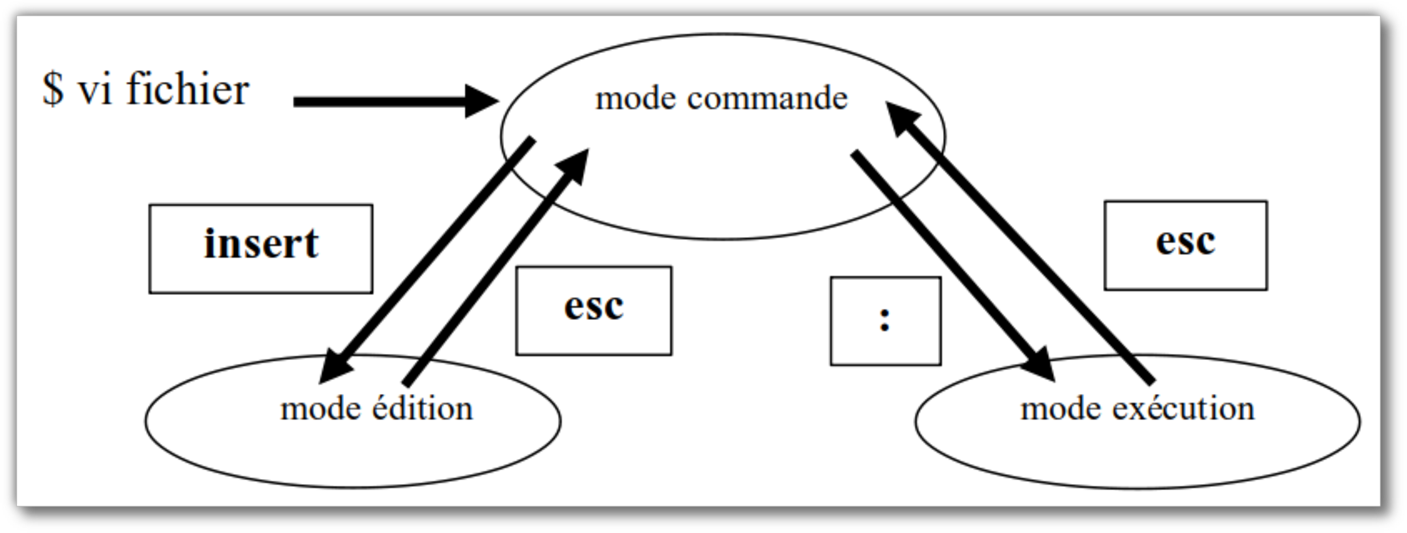
\includegraphics[width=.7\textwidth]{image/vi.pdf}
                \end{center}
    
            \subsubsection*{Le mode commande}
            %===============================
    
                C'est le mode dans lequel vous vous trouvez quand vous ouvrez \samp{vi}. 
                Dans ce mode, les touches sur lesquelles vous appuyez
                ne sont pas insérées dans le texte (comme dans nano)
                mais sont considérées comme des commandes.
                C'est le mode qui permet de \textbf{manipuler} le texte.
    
                Exemples de commandes :
                \begin{itemize}
                \item \kbd{i} : passer en mode édition (cfr. infra);
                \item \kbd{yy} : copier la ligne sous le curseur (comme un \samp{CTRL-C} sous Windows) ; 
                \item \kbd{3yy}	: copier 3 lignes ;
                \item \kbd{dd} : couper la ligne sous le curseur (\kbd{5yy} pour en couper 5) ;
                \item \kbd{dw} : couper le mot sur lequel se trouve le curseur ;
                \item \kbd{p} : coller (ce qui a été précédemment copié ou coupé)
                    sous la ligne qui suit le curseur ;
                \item \kbd{u} : annuler la dernière modification. 
                    Vous pouvez appuyer plusieurs fois pour annuler les dernières modifications.	
                \end{itemize}
    
                \subsubsection*{Le mode édition}
                %===============================
            
                    C'est le mode dans lequel ce qu'on tape est ajouté au texte,
                    comme dans nano.
                    On y accède par la touche :
                    \begin{itemize}
                    \item \kbd{i} (insert) : on insère à l'endroit du curseur ;
                    \item \kbd{a} (append) : on insère après le curseur ;
                    \item \kbd{o} : on insère dans une nouvelle ligne créée sous le curseur ;
                    \end{itemize}
    
                    Dans tous les cas, l'indicateur \texttt{INSERT} 
                    apparait alors en bas de l'écran.
    
                \subsubsection*{Le mode exécution}
                %===============================
                
                    On y accède à partir du mode commande en tapant \kbd{:}.
                    Ce mode permet d'entrer d'autres types de commandes,
                    plus riches que celles du mode commande. 
                    Voici les plus utilisées:
                    \begin{itemize}
                    \item \kbd{:h} pour accéder à l'aide (\kbd{q} pour quitter l'aide) ;
                    \item \kbd{:w} pour sauver le fichier ;
                    \item \kbd{:w monFichier} pour enregistrer sous \samp{monFichier},
                    \item \kbd{:q} pour quitter l'éditeur (sans sauver) ;
                    \item \kbd{:x} pour enregistrer et quitter ;
                    \item \kbd{:q!} pour quitter sans enregistrer les modifications ;
                    \item \kbd{:set nu} pour afficher les numéro de ligne 
                        (\kbd{:set nonu} pour les retirer) ;
                    \item \kbd{:numéroDeLigne} pour aller directement à cette ligne ;
                    \item \kbd{:\%s/old/new/g} 
                        pour remplacer toutes les occurrences de la chaine de caractères 
                        \samp{old} par la chaine de caractère \samp{new}.
                    \end{itemize}
    
        \subsection{Pour aller plus loin : le prompt}
        %=============================================
    
            \begin{Exercice}{Explorer les codes du prompt}
                Les possibilités de configuration du prompt sont nombreuses : 
                afficher l'heure, le nom de la machine, votre login,
                utiliser des couleurs\dots{}
                Examinez la documentation pour configurer le prompt comme il 
                vous plait (\verb@man bash@, section \verb@PROMPTING@).
                Rendez la modification permanente.
            \end{Exercice}	
            
\end{document}
